\section{Zielsetzung}
\label{sec:Zielsetzung}
In diesem Versuch sollen die Verdampfungswärme $L$ von Wasser und ihre Temperaturabhängigkeit bestimmt werden.\\
Außerdem wird die dazugehörige Dampfdruckkurve ermittelt.\\


\section{Theorie}
\label{sec:Theorie}

\subsection{Phasenübergänge}
\label{subsec:Phasenuebergaenge}
In welchem der drei Aggregatzustände sich ein Stoff befindet, hängt von 
der kinetischen Energie der Teilchen im Inneren ab. \\
Betrachtet man den Stoff als abgeschlossenes System, lässt sich dessen Zustand in zwei
Freiheitsgraden, Temperatur $T$ und Druck $p$ beschreiben. \\
In einem Phasendiagramm ist dargestellt, bei welchen Werten der beiden Parameter der Stoff welchen
Aggregatzustand annimmt. \\
In diesem Diagramm lassen sich zwei relevante Punkte ausmachen. Der kritische Punkt ist der Punkt, in dem zwischen den Zuständen 
flüssig und gasförmig nicht unterschieden werden kann. \\
Im sogenannten Tripel-Punkt liegen alle drei Aggregatzustände gleichzeitig vor. \\

\begin{figure}[H]
    \centering
    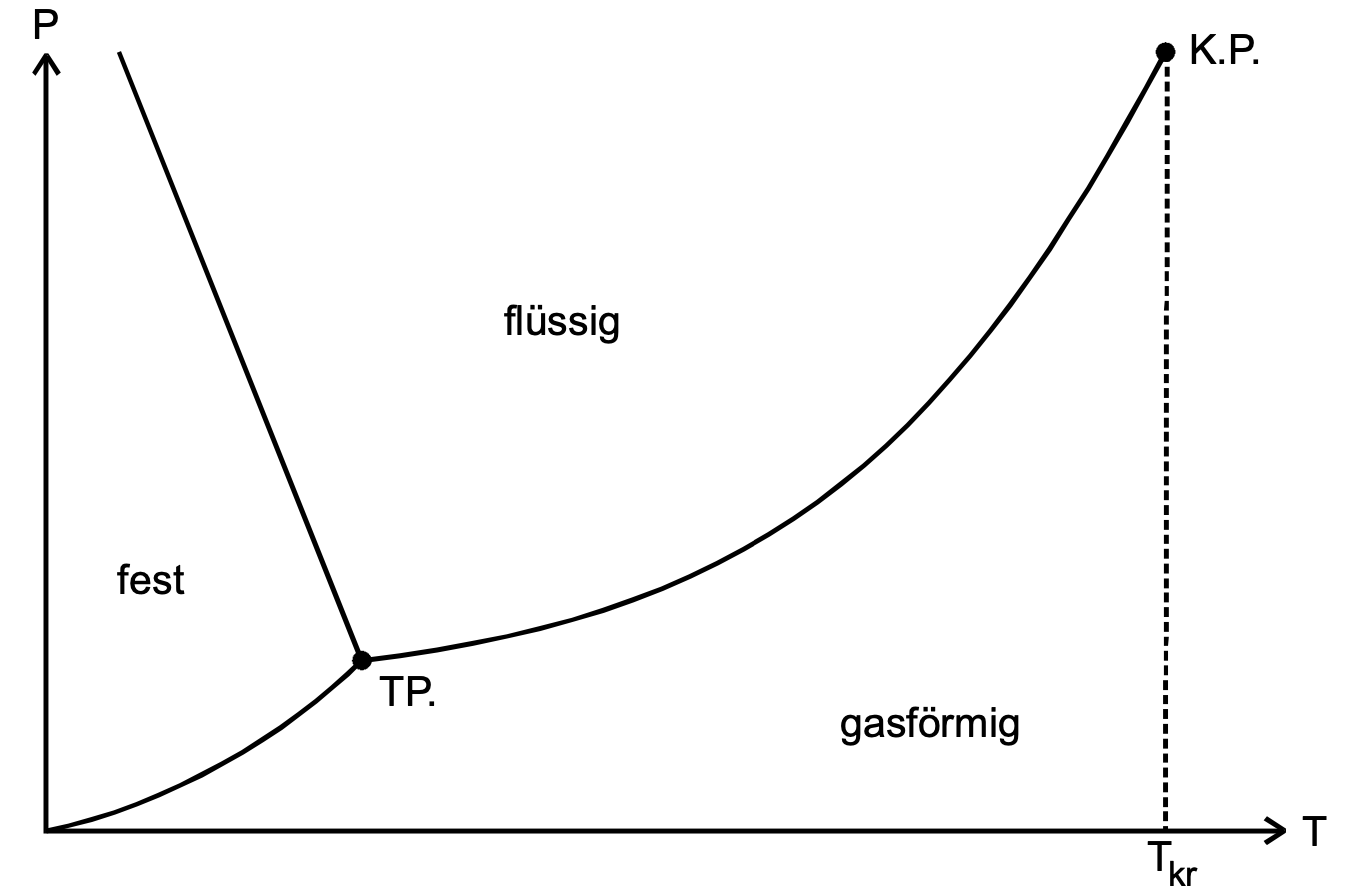
\includegraphics[scale=0.5]{content/v203_abb3.png}
    \caption{Die Dampfdruckkurve von Wasser. \cite{sample}}
    \label{abb:dampfkurve}
\end{figure}


\subsection{Dampfdruckkurve}
\label{subsec:Dampfdruckkurve}
Die Dampfdruckkurve ist von der molaren Verdampfungswärme $L$ abhängig.\\
$L$ ist eine charakteristische, temperaturabhängige Größe des Stoffes.\\
Sie gibt Auskunft darüber, welche Menge an Wärmeenergie nötig ist, damit 
ein Mol des Stoffes isotherm und isobar verdampfen zu lassen. \\
In der Umgebung des sogenannten Tripel-Punktes wird sie beinahe konstant. \\  
Die Energie, um zwischen den Phasen zu wechseln, muss dem System von außen zugeführt oder 
entzogen werden.\\
Der gesättigte Dampf lässt sich mit der allgmeinen Gasgleichung
\begin{equation}
    pV = RT
\label{eqn:allg_gasgl}
\end{equation}
beschreiben. Hier entspricht R der allgemeinen Gaskonstante $R = 8,134 \frac{J}{K\:mol}$. \\


\subsection{Clausius-Clapeyronsche Gleichung}
\label{subsec:Clausius-Clapeyron}
Bei Temperaturen, die weit unterhalb des kritischen Punktes des Stoffes liegen,
lassen sich einige Näherungen annehmen. \\
Und zwar:

\begin{enumerate}
    \item L ist nicht von Druck und Tempreratur abhängig
    \item Das Flüssigkeitsvolumen $V_F$ ist gegenüber dem Dampfvolumen $V_D$ vernachlässigbar
    \item Das Dampfvolumen $V_D$ darf durch die allgemeine Gasgleichung \autoref{eqn:allg_gasgl} beschrieben werden
\end{enumerate}